\chapter{TINJAUAN PUSTAKA}
\label{chap:tinjauanpustaka}


\section{Penelitian Terkait}
\label{sec:penelitianterdahulu}

\subsection{\textit{Smart Whiteboard for Interactive Learning}}
\label{subsec:smartwbforinteractivelearning}
Pada penelitian \textit{smart whiteboard for interactive learning} bertujuan untuk mencoba menyediakan suatu cara alternatif dan terjangkau pada papan tulis atau slides agar bisa mendapat interaksi lebih dari murid serta untuk meningkatkan efisiensi dari pengajaran. Pada penelitian ini, peneliti membuat sebuah papan tulis interaktif menggunakan Nintendo Wii \textit{Remote} dan \textit{PC Suite}. \textit{Software Suite} yang dikembangkan memungkinkan tampilan PC apapun dapat digunakan sebagai papan tulis interaktif. Sistem yang dibangun memiliki fungsi yang diperlukan untuk menciptakan sarana pembelajaran yang lebih baik dan lebih berteknologi, serta memberi pengguna dan siswa alat tambahan untuk menunjang Pendidikan interaktif. \textit{PC Suite} dibuat seramah mungkin sehingga dapat digunakan dengan mudah pada komputer spesifikasi standar. Pada konklusi penelitian, sistem yang telah dibuat telah memiliki fungsionalitas penuh yang diperlukan dalam membuat pembelajaran kelas lebih interaktif \citep*{kellerman2018smart}.  \par

\subsection{\textit{Handwritten Text Segmentation Using Pixel Based Approach}}
\label{subsec:handwrittenpixelbasedapproach}
Penelitian \textit{handwritten text segmentation using pixel based approach} menyajikan pendekatan sederhana untuk segmentasi huruf kata tulisan tangan menggunakan pendekatan bounding box dan pendekatan berbasis pixel. Segmentasi huruf tulisan tangan merupakan proses yang menantang karena gaya penulisan yang bervariasi. Kata-kata tulisan tangan yang tidak bersentuhan disegmentasikan dengan pendekatan bounding box dan kata-kata tulisan tangan yang bersentuhan disegmentasi menggunakan pendekatan pixel. Penelitian ini mencapai tingkat segmentasi hingga 94.45\% dan tingkat pengenalan 85.89\% dengan skema training dan testing 50-50\% \citep*{arun2019handwritten}. \par

\subsection{Pengenalan Objek Makanan Cepat Saji Pada Video dan \textit{Real Time} Webcam Menggunakan Metode \textit{You Only Look Once} (YOLO)}
\label{subsec:pengenalanobjekrealtime}
Pada penelitian ini, peneliti membuat pengenalan objek Makanan cepat saji dari \textit{video} dan \textit{real time webcam} menggunakan metode \textit{deep learning. You Only Look Once (YOLO)} merupakan model \textit{deep learning} yang digunakan untuk pengenalan objek. Jumlah data yang digunakan terdiri dari 468 gambar yang terdiri dari 3 jenis Makanan cepat saji yaitu \textit{hamburger, pizza, \textnormal{dan} hot dog}. Dari hasil penelitian, didapatkan hasil nilai avg loss pada model akhir yang dibangun yaitu 4.6\%, nilai validasi mAP 100\%, serta akurasi akhir berkisar antara 63\% sampai 100\% \citep*{karlina2020pengenalan}. \par

\subsection{\textit{Safety Helmet Detection Based on YOLOv5}}
\label{subsec:safetyhelmetyolov5}
Pada penelitian \textit{Safety Helmet Detection Based on YOLOv5} bertujuan untuk membuat deteksi helm keselamatan menggunakan YOLOv5 untuk membangun suatu sistem monitoring helm keselamatan \textit{digital.} Jumlah data yang digunakan yaitu 6045 citra dari internet yang kemudian diberi anotasi dan dibagi menjadi \textit{training set \textnormal{dan} testing set} dengan rasio 2:1. Pada proses \textit{training} menggunakan 2 jenis kelas dengan epochs 100, \textit{learning rate} 0.01, \textit{optimizer} SGD, \textit{batch-size} 16, dan \textit{image-size} 640*640. Pada proses \textit{training} dengan \textit{pretrained weight} YOLOv5s didapatkan mAP 0.936, YOLOv5m didapatkan mAP 0.943, YOLOv5l 0.944, dan YOLOv5x 0.947 \citep{zhou2021safety}. \par

% Per Teori Penunjang dibuat section baru

% papan tulis

% \section{Papan Tulis}
% \label{sec:papantulis}
% Papan tulis merupakan papan yang terbuat dari kayu dengan permukaan yang dapat ditulis ulang dengan menggunakan kapur tulis. Papan tulis awalnya dibuat dari lembaran tipis batu tulius berwarna hitam atau abu-abu.


\section{\textit{Citra}}
\label{sec:citra}

Citra atau gambar merupakan representasi visual dari suatu objek, orang, atau pemandangan. Secara umum, terdapat 2 jenis citra yaitu citra analog dan citra digital. Citra analog merupakan citra yang bersifat kontinyu dan tidak dapat direpresentasikan dalam komputer sehingga tidak dapat diproses oleh komputer secara langsung. Adapun untuk melakukan pemrosesanpada citra analog perlu dilakukan konversi dari analog menjadi digital \citep*{tyagi2018understanding}. \par

Citra digital terdiri dari elemen gambar yang juga dikenal sebagai piksel. Citra digital adalah fungsi 2 dimensi f(x,y) yang merupakan proyeksi pemandangan 3 dimensi kedalam bidang proyeksi 2 dimensi dimana x dan y mewakili lokasi piksel dan mengandung intensitas nilai. Adapun jika nilai x,y, dan intensitas bersifat diskrit, maka citra tersebut dapat dikatakan sebagai citra digital \citep*{tyagi2018understanding}. \par

\section{\textit{Image Processing}}
\label{sec:imageprocessing}
Citra direpresentasikan dalam bentuk matriks numerik yang memiliki informasi intensitas atau warna pada tiap elemen gambar. Karena itu operasi matematika sangat penting dalam berbagai proses pengolahan citra. Dalam pelaksanaan proses pengolahan citra, sebagian proses dilakukan dalam citra skala abu-abu (\textit{grayscale}). Adapun untuk pengolahan citra berwarna, mulanya citra berwarna tersebut dapat didekomposisi menjadi komponen merah, hijau, dan biru dan masing-masing komponen diproses secara independen sebagai citra \textit{grayscale} \citep*{tyagi2018understanding}. Secara umum, proses pengolahan citra terbagi menjadi 3 tingkatan sebagai berikut:
\begin{enumerate}[nolistsep]
    \item \textit{Low-Level Image Processing. \textnormal{Pada} low-level image processing, input \textnormal{dan} output} adalah berupa gambar dan proses yang dilakukan merupakan operasi sederhana. Adapun contoh dari \textit{low-level image processing} yaitu seperti \textit{contrast enhancement \textnormal{dan} noice reduction.}  
    \item \textit{Mid-Level Image Processing. \textnormal{Pada} mid-level image processing,} proses yang dilakukan merupakan operasi yang melibatkan ekstraksi atribut dari suatu citra. Adapun contoh dari \textit{mid-level image processing \textnormal{yaitu seperti} Edges, Contours, \textnormal{dan} Regions.}
    \item \textit{High-Level Image Processing. \textnormal{Pada} high-level image processing,} proses yang dilakukan merupakan operasi kompleks yang berkaitan dengan analisis dan interpretasi konten untuk pengambilan keputusan.
\end{enumerate} 

\section{\textit{Deep Learning}}
\label{sec:deeplearning}
\textit{Deep learning} adalah serangkaian algoritma dalam \textit{machine learning} yang mempelajari fitur-fitur dari sebuah data mentah secara otomatis. \textit{Deep learning} merupakan cabang dari \textit{machine learning} yang didasarkan pada \textit{artificial neural network}. \textit{Artificial neural network} terinspirasi dari arsitektur saraf otak manusia, dan seperti halnya otak manusia, \textit{artificial neural network} terdiri dari berbagai neuron. Seperti \textit{neural network} tradisional, \textit{deep neural network} juga terdiri dari neuron buatan yang disusun dalam bentuk \textit{input layer, hidden layer, \textnormal{dan} output layer}. Namun, tidak seperti \textit{neural network} tradisional, jumlah \textit{hidden layer \textnormal{pada} deep neural network} umumnya terdiri lebih dari 1 \textit{layer} \citep*{ahmad2019deep}. 
% \textit{Deep learning} memungkinkan model komputasi dari beberapa lapisan pemrosesan untuk mempelajari dan mewakili data dengan berbagai tingkat abstraksi. 
% \textit{Deep learning} merupakan metode yang memiliki implementasi sangat banyak mencakup \textit{neural Networks, hierarchical probabilistic models, unsupervised learning} dan \textit{supervised learning} \citep*{voulodimos2018deep}. 
\textit{Deep learning} dirancang untuk dapat terus mengolah data dan menganalisa data tersebut seperti dalam mengambil keputusan. 
Adapun dalam \textit{deep learning, training} suatu data dipengaruhi oleh banyaknya jumlah layer dan jumlah neuron. Artinya, semakin banyak layer atau neuron yang digunakan maka akan semakin lama proses yang dilakukan, hal ini disebabkan oleh tingkat kompleksitas yang semakin besar juga. Ilustrasi \textit{layer \textnormal{pada} deep learning} dapat dilihat pada Gambar \ref*{fig:deeplearninglayer}. \par

\begin{figure}[H]
    \centering
    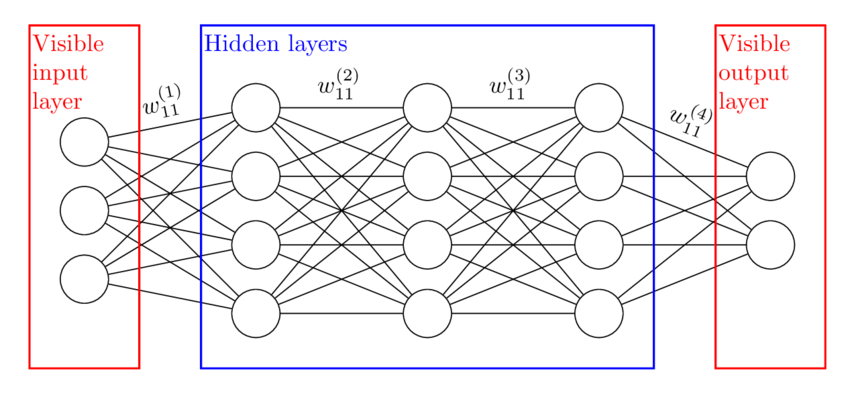
\includegraphics[scale=0.5]{gambar/deep learning layer.png}
    \caption{Ilustrasi \textit{Layer} pada \textit{Deep Learning}.}
    \label{fig:deeplearninglayer}
\end{figure}

Seperti \textit{machine learning, deep learning} juga memiliki beragam pendekatan dalam mempelajari suatu dataset. Secara umum, pendekatan \textit{deep learning} dapat dikategorikan kedalam 3 kelompok yaitu: \textit{Deep network for supervised learning, Deep Network for unsupervised learning,} dan hybrid. Adapun pada penelitian ini menggunakan CNN yaitu pendekatan dengan \textit{deep network for supervised learning,} hal ini dapat terlihat terlihat dari input dataset yang akan dilatih telah memiliki label atau kelas yang menunjukkan klasifikasi. Penjelasan mengenai kategori umum pendekatan dengan \textit{deep learning} yaitu sebagai berikut \citep*{ahmad2019deep}: \par

\begin{enumerate}[nolistsep]
    \item \textit{\textbf{Deep Network for Supervised Learning.} Deep network for supervised learning} mencoba untuk mempelajari perbedaan antara item data milik berbagai kelas dengan berdasarkan label yang telah diberikan dengan data. Dalam tugas klasifikasi dan regresi, \textit{deep network} mencoba untuk memetakan input ke \textit{output} yang diharapkan (label). Adapun arsitektur yang umum digunakan dalam \textit{supervised learning} yaitu \textit{Deep Neural Network (DNN), Convolutional Neural Network (CNN), \textnormal{dan} Recurrent Neural Network (RNN).} DNN memiliki struktur paling sederhana karena DNN merupakan \textit{feed forward neural network.}
    \item \textit{\textbf{Deep Network for Unsupervised Learning.} Unsupervised learning} mengacu pada metode \textit{learning} dimana informasi (label) tidak tersedia saat proses \textit{learning} dilakukan. Adapun metode paling umum dalam \textit{unsupervise learning} yaitu diantaranya \textit{deep autoencoder \textnormal{dan} deep Boltzmann machines (DBM).}
    \item \textit{\textbf{Hybrid.}} Pada metode hibrida yaitu menggabungkan antara metode \textit{supervised learning \textnormal{dan} unsupervised learning.} Pada pendekatan hibrida, sejumlah data tanpa label yang sangat besar misalnya, dapat menggunakan metode \textit{unsupervised learning} untuk mempelajari parameter awal untuk proses \textit{supervised learning} selanjutnya.  
\end{enumerate}

Adapun dalam membangun suatu algoritma \textit{deep learning,} terdapat beberapa istilah umum yang perlu diperhatikan, yaitu:
\begin{itemize}[nolistsep]
    \item \textit{\textbf{Layers.} Layer \textnormal{dalam model} deep learning} merupakan  suatu struktur atau topologi jaringan dalam arsitektur model yang mengambil informasi dari \textit{layer} sebelumnya dan kemudian meneruskan informasi ke \textit{layer} selanjutnya. Secara umum, pada \textit{deep learning} terdapat 3 jenis \textit{layer} yaitu \textit{input layer, hidden layer, \textnormal{dan} output layer.} Ada beberapa istilah \textit{layer} yang sering digunakan, khususnya dalam konteks \textit{hidden layer} diantaranya \textit{convolutional layers, pooling layer, \textnormal{dan} dense layer.}
    \item \textit{\textbf{Activation.} Activation} merupakan suatu fungsi yang ditambahkan di akhir \textit{output \textnormal{dari} neural network. Activation} digunakan untuk menentukan \textit{output neural network. Activation} secara umum terbagi menjadi 2 tipe yaitu \textit{linear \textnormal{dan} non linear.} 
    \item \textit{\textbf{Hyperparameter.} Hyperparameter} adalah parameter yang nilainya telah ditetapkan sebelum melakukan proses \textit{training} model. \textit{Hyperparameter} secara umum berbeda dengan parameter, karena parameter merupakan istilah untuk mengidentifikasi variabel yang nilainya didapat selama proses \textit{learning/training.} Penambahan \textit{"hyper" \textnormal{pada} "hyperparameter"} memiliki makna bahwa parameter memiliki tingkatan lebih tinggi yaitu untuk mengatur proses \textit{learning.} Contoh dari \textit{hyperparameter \textnormal{diantaranya yaitu} epochs, learning rate, batch-size, optimizer, loss function, \textnormal{dan} image-size.}
    \item \textit{\textbf{Evaluation Metrics.} Evaluation metrics} atau matriks evaluasi merupakan matriks yang digunakan untuk melakukan evaluasi pada suatu model yang sebelumnya telah dilakukan proses \textit{training.} Beberapa contoh jenis dari matriks evaluasi diantaranya yaitu \textit{accuracy, recall, precision, f1 scores, log loss/binary crossentropy, confusion matrix, intersect over union (IoU), \textnormal{dan} mean average precision.}
\end{itemize}

\section{\textit{Object Detection}}
\label{sec:objectdetection}

\textit{Object detection} merupakan teknik dalam visi komputer yang berfungsi untuk mengidentifikasi dan menemukan objek dari suatu citra gambar ataupun video. Secara spesifik, \textit{object detection} menggambar \textit{bounding box} disekitar objek yang dideteksi, sehingga memungkinkan pengembang untuk menentukan lokasi objek tersebut dalam suatu skenario. Pendekatan umum dari  \textit{frameworks} deteksi objek mencakupi pembuatan set besar yang diklasifikasikan secara sekuel menggunakan fitur CNN \citep*{voulodimos2018deep}. \par

\textit{Object detection} seringkali disalah artikan sebagai \textit{image recognition. Image recognition} contohnya, pada sebuah citra berisikan objek anjing akan mendapatkan label 'anjing', jika dalam sebuah citra berisikan objek 2 anjing maka tetap akan mendapatkan label 'anjing'. Disisi lain, \textit{object detection} menggambar \textit{bounding box} pada tiap objek anjing dan memberikan label pada \textit{bounding box} tersebut dengan label 'anjing'. Perbedaan antara \textit{object detection \textnormal{dan} image recognition} secara sederhana dapat dilihat pada Gambar berikut. 
\par

\begin{figure}[H]
    \centering
    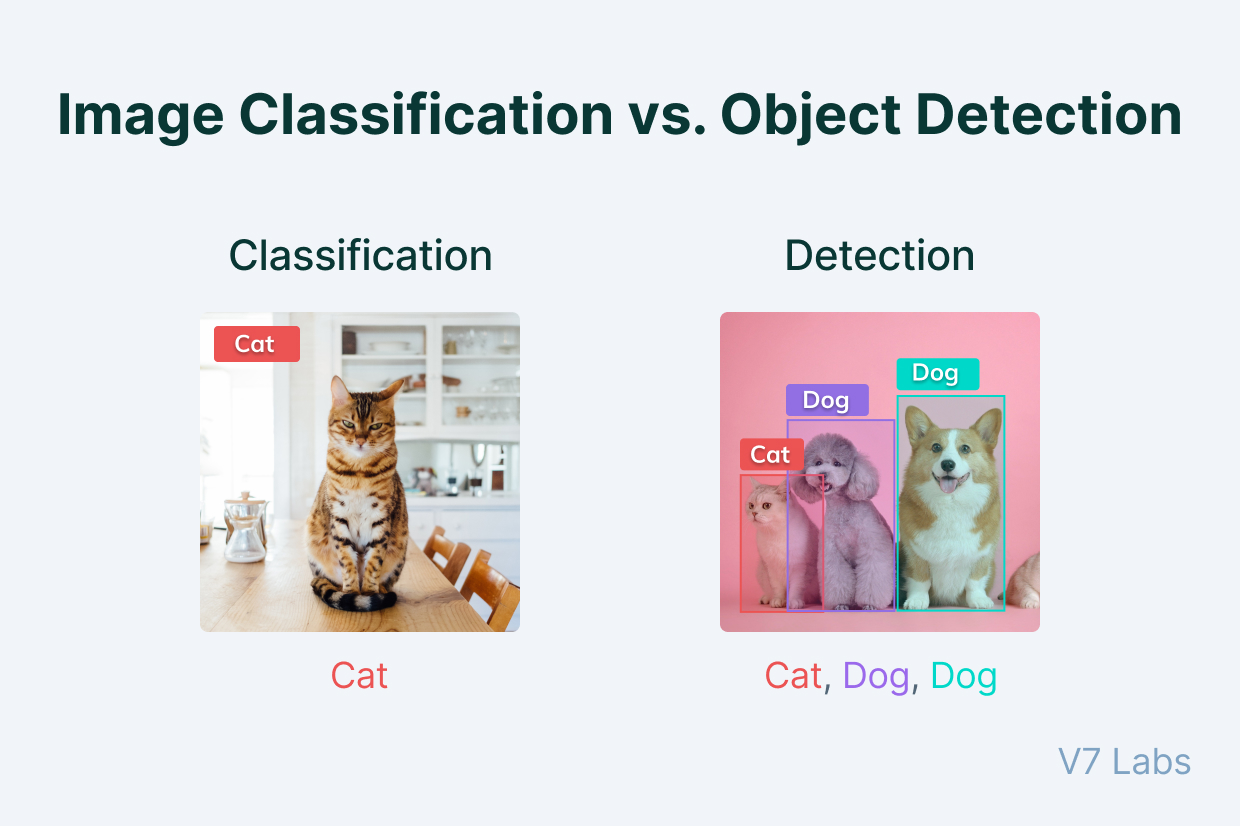
\includegraphics[scale=0.5]{gambar/object_detection_vs_image_recognition.jpg}
    \caption{Ilustrasi Perbedaan Antara \textit{Object Detection} dan \textit{Image Recognition \citep*{rizzoli_2022}.}}
    \label{fig:objectdetcompare}
\end{figure}

\section{\textit{Convolutional Neural Network (CNN)}}
\label{sec:convolutionalneuralnetwork}
CNN merupakan algoritma \textit{deep learning} yang mampu mengambil masukan berupa gambar, menetapkan prioritas untuk berbagai aspek/objek dalam gambar dan mampu membedakan satu sama lain. Tahapan \textit{pre-processing} yang dibutuhkan CNN lebih sedikit jika dibandingkan dengan algoritma klasifikasi lainnya \citep*{towardsDS}. \textit{Convolutional Neural Network (CNN)} itu sendiri juga merupakan pengembangan dari \textit{Multilayer Percepton (MLP)} yang didesain untuk mengolah data dua dimensi. CNN termasuk dalam jenis \textit{Deep Neural Network} karena kedalaman jaringan yang tinggi dan banyak diaplikasikan pada data citra \citep*{putra2016klasifikasi}.\par

Secara umum, cara kerja CNN hampir serupa pada MLP, hanya saja dalam CNN setiap neuron dipresentasikan dalam bentuk dua dimensi. Adapun cara kerja dari suatu MLP sederhana yaitu MLP semula memiliki sejumlah \textit{layer} dengan masing-masing layer memiliki sejumlah \textit{neuron}. MLP menerima masukan data dalam bentuk satu dimensi, kemudian mempropagasikan data tersebut pada jaringan sehingga didapat hasil keluaran. Setiap hubungan antar \textit{neuron} pada dua \textit{layer} yang bersebelahan memiliki parameter bobot satu dimensi yang menentukan kualitas mode. Disetiap data input pada layer dilakukan operasi linear dengan nilai bobot yang ada, kemudian hasil komputasi akan ditransformasi menggunakan operasi non linear yang disebut sebagai fungsi aktivasi. \par

CNN memiliki beberapa jenis \textit{neural layers} utama yang masing-masing memiliki peranannya masing-masing \citep*{voulodimos2018deep}. Adapun secara sederhana, CNN terdiri dari 3 jenis utama \textit{neural layers} yaitu: \par
\begin{enumerate}[nolistsep]
    \item \textit{Convolutional Layer}
    \item \textit{Pooling Layer}
    \item \textit{Fully Connected Layer}
\end{enumerate}
\par

\subsection{\textit{Convolutional Layer}}
\label{subsec:convlayer}

\textit{Convolutional Layer} atau lapisan konvolusi merupakan lapisan inti dari sebuah arsitektur CNN dan juga merupakan pusat dimana sebagian besar proses komputasi terjadi. Konvolusi mengaplikasikan suatu fungsi pada \textit{output} fungsi lain secara berulang. Pada konvolusi, prosesnya menguji keberadaan fitur pada suatu citra tertentu dan kemudian CNN akan mencoba seluruh kemungkinan posisi pada citra tersebut. Beberapa macam fungsi yang sering digunakan dalam penelitian adalah \textit{sigmoid, tanh, Rectified Linear Unit (ReLU), Leaky ReLU (LReLU), \textnormal{dan} Parametric ReLU.}

\subsection{\textit{Pooling Layer}}
\label{subsec:poolinglayer}

Konsep utama dari \textit{pooling} yaitu melakukan \textit{down sampling} dalam rangka untuk mengurangi kompleksitas layer selanjutnya, atau dalam istilah pemrosesan citra seperti halnya proses mengurangi resolusi citra. \textit{Pooling} bertujuan untuk memperkecil ukuran citra berukuran besar tanpa mengurangi informasi-informasi penting didalamnya \citep*{Pangestu2018-mq}. \textit{Pooling} tidak mempengaruhi jumlah filter. Adapun metode yang umum digunakan dalam \textit{pooling} yaitu \textit{max-pooling} \citep*{8308186}. Pada \textit{max pooling} akan membagi \textit{output} dari layer sebelumnya menjadi beberapa grid kecil, lalu akan diambil nilai yang paling besar dari grid untuk dibuat matriks barunya. Ilustrasi \textit{max pooling layer} dapat dilihat pada Gambar \ref*{fig:poolinglayer} berikut.

\begin{figure}[H]
    \centering
    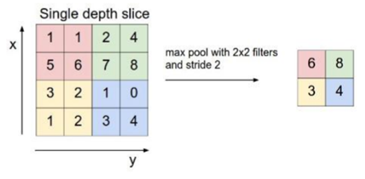
\includegraphics[scale=0.9]{gambar/poolinglayer.png}
    \caption{Ilustrasi \textit{Max Pooling Layer} \citep*{poolinglayer}}
    \label{fig:poolinglayer}
\end{figure}

\subsection{\textit{Fully Connected Layer}}
\label{subsec:fullyconnectedlayer}

\textit{Fully connected layer} memiliki tugas untuk melakukan klasifikasi berdasarkan fitur yang diekstraksi pada  layer sebelumnya dan filter yang berbeda. \textit{Fully connected layer} memiliki cara kerja serupa seperti cara neuron diatur dalam suatu ANN. Setiap node dalam suatu \textit{fully connected layer} terhubung langsung ke seluruh node baik itu di \textit{layer} sebelumnya ataupun \textit{layer} setelahnya \citep*{8308186}.

\section{\textit{Region Based Convolutional Neural Network (R-CNN)}}
\label{sec:regionbasedconvolutionalneuralnetwork}

Visi komputer merupakan bidang interdisipliner yang mendapatkan daya tarik cukup besar dalam beberapa tahun terakhir sejak CNN dan mobil \textit{self driving} menjadi popular. \textit{Object detection} merupakan salah satu bagian penting dalam visi komputer. Perbedaan antara deteksi dan klasifikasi yaitu pada algoritma deteksi, \textit{bounding box} diberikan disekitar objek pada suatu citra. Selain itu, pada algoritma deteksi tidak menutup kemungkinan bahwa dalam satu citra terdapat lebih dari 1 objek yang merepresentasikan objek lain ataupun objek serupa dalam satu citra. Pada kondisi inilah, permasalahan ini tidak dapat diselesaikan hanya dengan membangun suatu model CNN standar dikarenakan jumlah objek yang terdapat dalam suatu citra tidak menentu \citep*{Girshick_2014_CVPR}. \par

Salah satu pendekatan yang dapat dilakukan untuk menyelesaikan permasalahan tersebut yaitu dengan mengambil beberapa \textit{region of interest} berbeda dari suatu citra, dan menggunakan CNN untuk melakukan klasifikasi objek didalam area \textit{region} tersebut. Kemudian permasalahan lain yang akan dihadapi jika menggunakan pendekatan ini adalah \textit{region of interest} pada tiap citra mungkin memiliki lokasi yang berbeda dan jika tetap dilakukan komputasi maka akan berdampak buruk pada perangkat keras komputasinya. \par

Untuk mengatasi permasalahan tersebut, Ross Girshick dan rekannya menawarkan metode R-CNN dimana menggunakan \textit{selective search} untuk melakukan ekstraksi pada 2000 \textit{region} dari citra yang disebut juga dengan \textit{region proposal.} Sehingga, alih-alih mencoba untuk melakukan klasifikasi pada \textit{region} dalam jumlah besar tak menentu, prosesnya dibatasi hanya sampai 2000 \textit{region.}

\begin{figure}[H]
    \centering
    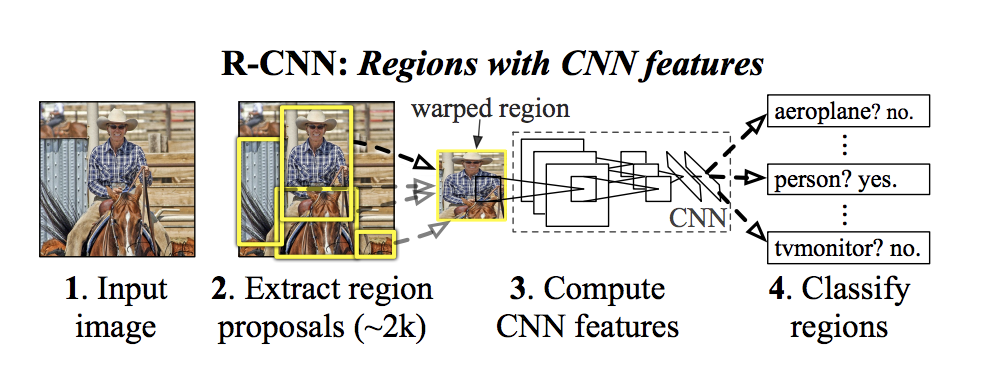
\includegraphics[scale=0.4]{gambar/rcnn.png}
    \caption{Ilustrasi R-CNN: \textit{Regions \textnormal{dengan} CNN features} \citep*{Girshick_2014_CVPR}}
    \label{fig:ilustrasircnn}
\end{figure}


\section{\textit{Evaluation Metrics}}
\label{sec:evaluationmetrics}

\textit{Evaluation metrics} merupakan matriks yang biasa digunakan dalam \textit{machine learning \textnormal{atau} deep learning} untuk mengukur kualitas model secara statistika. Terdapat berbagai jenis \textit{evaluation metrics} yang dapat digunakan sesuai dengan kebutuhan diantaranya seperti \textit{classification accuracy, logarithmic loss, \textnormal{dan} confusion matrix.}

\subsection{\textit{Precision}}
\label{subsec:precision}

\textit{Precision} merupakan nilai yang dapat didapatkan dengan cara membagi jumlah total contoh positif yang diklasifikasikan dengan benar dengan jumlah total contoh positif yang diprediksi. \textit{Precision} memenuhi Persamaan \ref*{eq:precision} berikut \citep*{hanafi2020deteksi}. \par

\begin{equation}
    \label{eq:precision}
    Precision=\frac{TP}{TP + FP}
\end{equation}

\subsection{\textit{Recall}}
\label{subsec:recall}

\textit{Recall} dapat diartikan sebagai rasio dari jumlah total contoh positif yang diklasifikasikan dengan benar dibagi dengan jumlah total contoh positif. \textit{High recall} yaitu merupakan kondisi dimana kelas dikenali dengan benar (\textit{false negative} sedikit). Adapun \textit{recall} memenuhi Persamaan \ref*{eq:recall} berikut.

\begin{equation}
    \label{eq:recall}
    Recall=\frac{TP}{TP + FN}
\end{equation}

\subsection{\textit{Mean Average Precision (mAP)}}
\label{subsec:meanaverageprecision}

\textit{Mean average precision} (mAP) merupakan nilai rata-rata dari \textit{average precision (AP)} yang membentuk matriks evaluasi untuk mengukur kinerja dari sebuah deteksi objek. Adapun nilai mAP didapatkan dari perhitungan \textit{precision.}

\subsection{\textit{Confusion Matrix}}
\label{subsec:confusionmetrics}

\textit{Confusion Matrix} merupakan salah satu metode untuk mengetahui seberapa baik model \textit{machine learning} yang dibuat. Dalam \textit{confusion matrix} terdapat beberapa istilah yaitu:
\begin{enumerate}[nolistsep]
    \item \textit{\textbf{True Positive.} True positive} berarti suatu model memprediksi data pada kelas positif dan data yang sebenarnya berada pada kelas positif.
    \item \textit{\textbf{True negative.} True negative} berarti suatu model memprediksi data pada kelas negatif dan data yang sebenarnya berada pada kelas positif.
    \item \textit{\textbf{False Positive.} False positive} berarti suatu model memprediksi data ada di kelas negatif dan data yang sebenarnya berada pada kelas negatif.
    \item \textit{\textbf{False Negative.} False negative} berarti suatu model memprediksi data ada di kelas negatif dan data yang sebenarnya berada pada kelas negatif.
\end{enumerate}

% \subsection{F1 \textit{Scores}}
% \label{subsec:f1scores}

% \subsection{\textit{Intersect over Union (IoU)}}
% \label{subsec:intersectoverunion}

% keknya gaperlu ??
% \section{Word Segmentation}
% \label{sec:wordsegmentation}
% Pengenalan tulisan tangan merupakan Teknik untuk menginterpretasikan tulisan tangan kedalam bentuk digital. Proses pengenalan tulisan tangan dapat diperoleh dengan 2 cara yaitu dengan mengonversi otomatis karakter pada saat ditulis pada layar sentuh dengan pena digital dan cara lain yaitu dengan melakukan pengambilan gambar serta pemrosesan gambar pada suatu teks yang ingin dikenali [8]. Pada proses segmentasi huruf, mulanya dokumen gambar disegmentasi kedalam baris-baris teks. Kemudian, algoritma segmentasi huruf diterapkan pada satu baris teks tersebut. Pada satu baris teks tersebut, secara umum proses segmentasi huruf konvensional menjalankan algoritma yang terdiri dari 2 tahapan yaitu: ekstraksi kandidat huruf berdasarkan pemisah huruf dan dilanjut dengan klasifikasi kandidat huruf \citep*{ryu2015word}.

\section{\textit{You Only Look Once (YOLO)}}
\label{sec:yolo}
YOLO merupakan salah satu algoritma pendeteksi objek yang dicetuskan oleh Redmon et al pada tahun 2015 lewat paper yang berjudul \textit{You Only Look Once: Unified, Real-Time Object Detection.} YOLO menggunakan basis sistem arsitektur yaitu CNN yang dioptimasi untuk mendeteksi objek pada gambar. Arsitektur YOLO sangat cepat apabila dibandingkan dengan arsitektur pengenalan objek lainnya. YOLO melakukan pendekatan ulang pada deteksi objek sebagai sebuah regresi tunggal \citep*{redmon2016you}. \par

% YOLO melakukan proses pengenalan objek berbasis CNN dalam sebuah kotak yang disebut \textit{anchor} yang dipusatkan pada 13x13 \textit{grid cell} dalam sebuah gambar. Artinya, ukuran gambar diubah (dikurangi) menjadi 416x416 terlepas dari ukuran asli dari gambar yang ingin di proses \textit{train or detect}. Artinya, jika terdapat perbedaan besar dalam rasio gambar yang diproses \textit{train}, maka akan terjadi distorsi serius pada objek ketika dilakukan proses penyesuaian ukuran\citep*{jeong2018image}. \par

\subsection{YOLOv5}
\label{subsec:yolov5}

YOLOv5 merupakan versi pembaruan dari YOLO yang dicetuskan oleh Glen Jocher pada tahun 2020. YOLOv5 diluncurkan tidak lama setelah perilisan YOLOv4. YOLOv5 diperkenalkan menggunakan \textit{framweork} Pytorch. YOLOv5 terdiri dari 3 bagian utama yaitu \textit{Backbone, Neck, \textnormal{dan} Head.} Bagian \textit{backbone} YOLOv5 menggunakan CSP-Darknet53, bagian \textit{neck} YOLOv5 menggunakan SPPF dan CSP-PAN, sedangkan pada bagian \textit{head} YOLOv5 menggunakan YOLOv3 \textit{Head} \citep*{ultralyticsyolo}. Struktur YOLOv5 secara umum dapat dilihat pada Gambar \ref{fig:strukturyolov5}. \par

\begin{figure}[H]
    \centering
    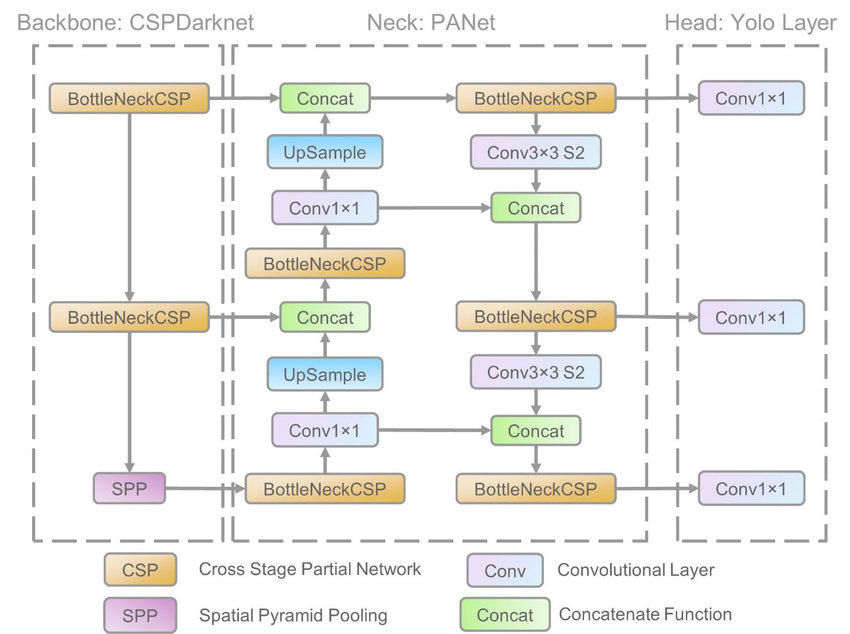
\includegraphics[scale=0.55]{gambar/yolov5.png}
    \caption{Struktur YOLOv5 \citep*{article}}
    \label{fig:strukturyolov5}
\end{figure}

Dalam pembuatan dataset untuk model YOLOv5, terdapat rekomendasi untuk jumlah data yang digunakan agar mendapatkan hasil yang optimal. Adapun rekomendasi tersebut yaitu \citep{ultralyticsyolo}:
\begin{enumerate}[nolistsep]
    \item \textit{\textbf{Image per Class.} Image per class} merupakan jumlah citra yang terdapat dalam suatu kelas terlepas dari pembagian \textit{training set, testing set \textnormal{ataupun} validation set.} Adapun rekomendasi yang dianjurkan yaitu tiap kelas memiliki jumlah citra sebanyak 1500 gambar atau lebih.
    \item \textit{\textbf{Instance per Class.} Instance per class} merupakan jumlah objek yang telah diberi label dalam suatu kelas. Adapun rekomendasi yang dianjurkan yaitu tiap kelas memiliki \textit{instance} sebanyak 10000 objek atau lebih.
    \item \textit{\textbf{Image Variety.} Image Variety} yaitu variasi citra dalam suatu kelas. Artinya sebuah citra dalam dataset sebaiknya representatif terhadap keadaan nyata \textit{(real world scenario).} Variasi citra dapat berupa variasi berdasarkan waktu ataupun musim pengambilan gambar, variasi pencahayaan gambar, variasi sudut pengambilan gambar, variasi sumber gambar.
\end{enumerate}
% //TODO: tabel comparison yolov5
